Since we decided to operate directly in MongoDB thorugh the provided shell, all the queries that we performed are written in MongoDB's query language. \\

As one can expect, since the most interesting information can be extracted by means of general statistic computed over the dataset, all of the queries that we performed are aggregate queries based on the \texttt{\$group} operator, which allows to group documents by a specific field and perform some operations on the grouped documents, such as counting them or computing the average of a specific field.

For this reason we decided to include some additional normal queries (mostly countDocuments() queries) to support our analysis where we thought it was necessary. \\

\newpage
\subsection{Order Products by Average Rating}
The most straightforward query that can be performed is to order the products by their average rating, in order to understand which are the most appreciated ones. \\
\begin{lstlisting}[language=Java]
db.reviews.aggregate([
  { $group: { _id: "$asin", avg_rating: { $avg: "$overall" } } },
  { $sort: { avg_rating: -1 } }
]);
\end{lstlisting}
Results:
\begin{figure}[H]
  \centering
  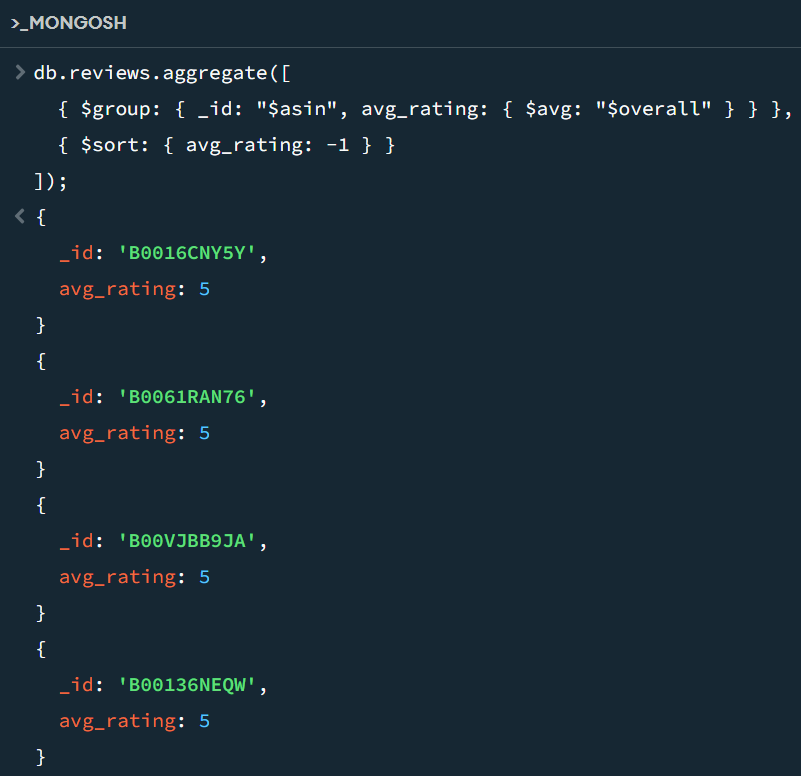
\includegraphics[scale=0.6]{Images/q1_result.png}
  \caption{Query 1 (partial) results}
  \label{fig:q1_result}
\end{figure}
As we can see from Figure \ref{fig:q1_result}, there are many products sharing the highest value for average rating, meaning that all the reviews that involve those products have the highest possible value, which is 5.\\

\subsection{Most Reviewed Products}
Another interesting query is to find the most reviewed products, in order to understand which are the most popular ones. \\
\begin{lstlisting}[language=Java]
db.reviews.aggregate([
  { $group: { _id: "$asin", count: { $sum: 1 } } },
  { $sort: { count: -1 } }
]);
\end{lstlisting}
Results:
\begin{figure}[H]
  \centering
  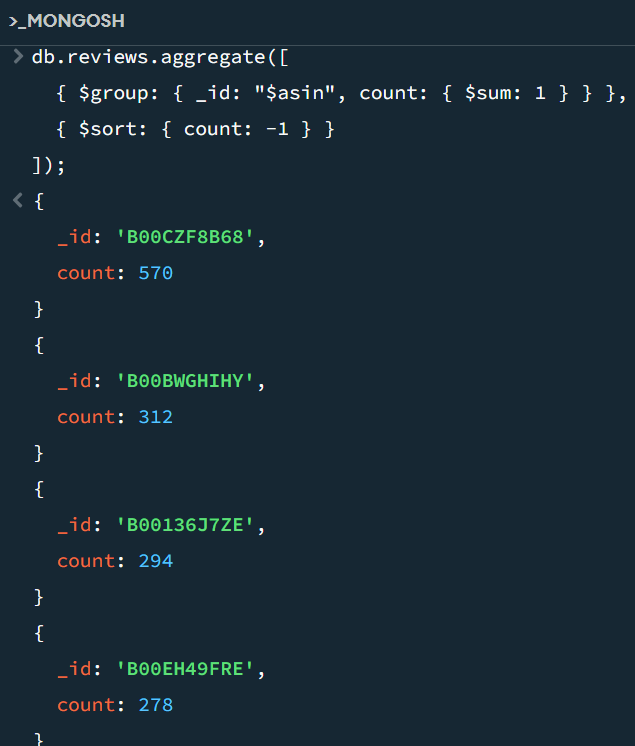
\includegraphics[scale=0.6]{Images/q2_result.png}
  \caption{Query 2 (partial) results}
  \label{fig:q2_result}
\end{figure}

\newpage
\subsection{Average Helpful Votes per Reviewer}
We can write a query to find the average number of helpful votes per reviewer, in order to understand which are the most appreciated ones. \\
\begin{lstlisting}[language=Java]
db.reviews.aggregate([
  { $group: { _id: "$reviewerID", 
    avg_votes: { $avg: {$ifNull:[{$toInt: "$vote"}, 0]} } } },
  { $sort: { avg_votes: -1 } }
]);
\end{lstlisting}
In this case we decided to use the \texttt{\$ifNull} operator to handle the case in which the \texttt{vote} field is missing: in practice, we filled the missing values in this field by putting them equal to 0. \\
Results:
\begin{figure}[H]
  \centering
  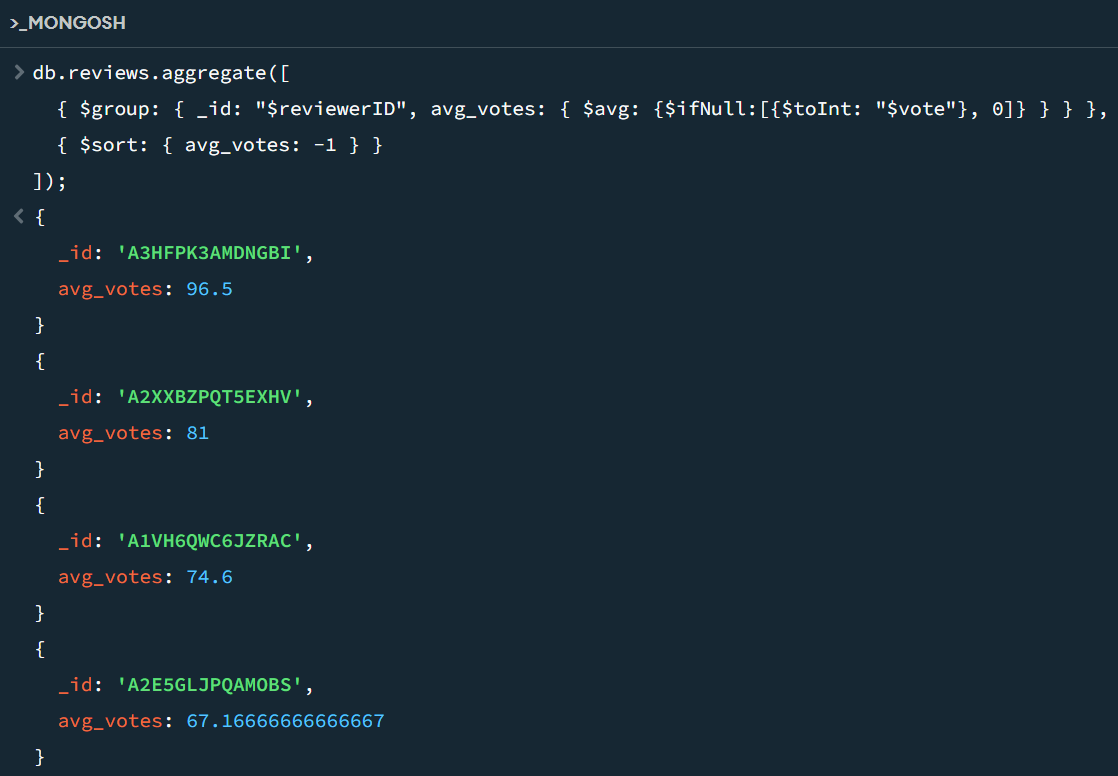
\includegraphics[scale=0.6]{Images/q3_result.png}
  \caption{Query 3 (partial) results}
  \label{fig:q3_result}
\end{figure}

\newpage
\subsection{Number of Reviews with Images per Verified Status}
Another aspect that could be useful is to compute the number of reviews that have at least one image attached for every possible value of the \textit{verified} field: this can be interesting since it can highlight a correlation between the fact that a purchase has been verified and the fact that some images were included in the relative review. \\
\begin{lstlisting}[language=Java]
db.reviews.aggregate([
  { $match: { image: { $exists: true } } },
  { $group: { _id: "$verified", count: { $sum: 1 } } }
]);
\end{lstlisting}
Results:
\begin{figure}[H]
  \centering
  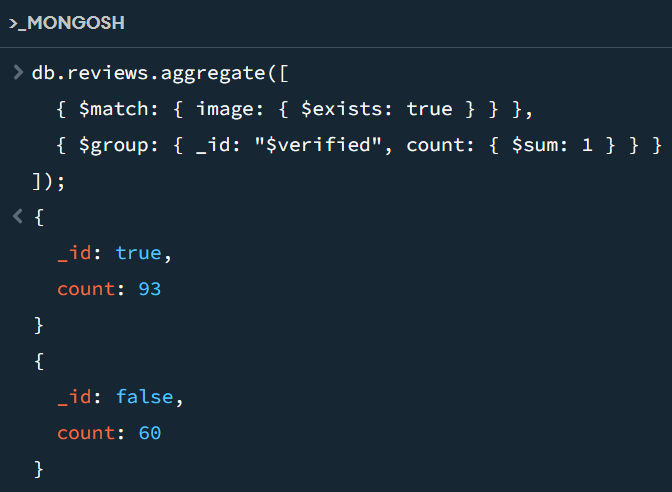
\includegraphics[scale=1]{Images/q4_result.png}
  \caption{Query 4 results}
  \label{fig:q4_result}
\end{figure}
From this output we can understand that the number of validated reviews with images is not so much higher than the other one, meaning that the presence of images is a not so strong indicator of the fact that the relative purchase has been verified. \\

\subsection{Temporal Distribution of Reviews}
It could be useful to look at the temporal distribution of reviews, in order to understand how the number of reviews has changed over time. \\
\begin{lstlisting}[language=Java]
db.reviews.aggregate([
  { $group: 
    { _id: 
      { year: { $year: { $toDate: {$multiply: [
          {
            "$toDecimal": "$unixReviewTime",
            
          },
          1000
        ]} } }, 
        month: { $month: { $toDate: {$multiply: [
          {
            "$toDecimal": "$unixReviewTime",
            
          },
          1000
        ]} } } }, 
      count: { $sum: 1 } } },
  { $sort: { "_id.year": -1, "_id.month": 1 } }
]);
\end{lstlisting}
Results:
\begin{figure}[H]
  \centering
  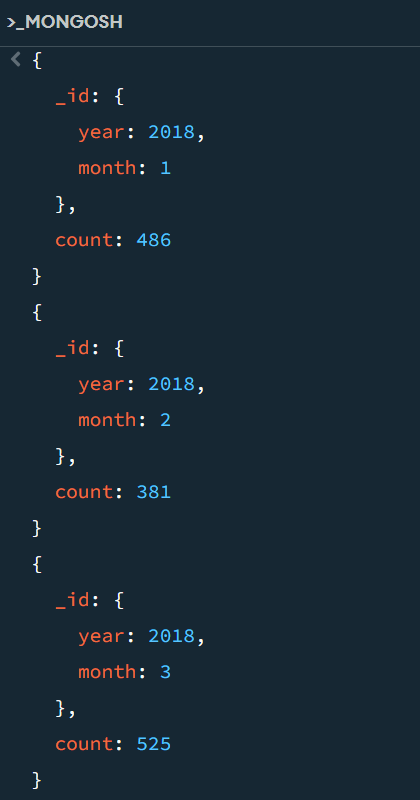
\includegraphics[scale=0.45]{Images/q5_result.png}
  \caption{Query 5 (partial) results}
  \label{fig:q5_result}
\end{figure}
\newpage
This query allows us to make multiple considerations:
\begin{itemize}
    \item the number of reviews has increased over the years: this can be easily explained by the fact that the dataset contains reviews from 1996 to 2018 and during this span of time the number of customers of the company has increased;
    \item the number of reviews is not constant inside the same year, but it has some peaks and some valleys: this can be explained by the fact that the amount of purchases is not constant during the year, but it is higher in some periods (e.g. Christmas) and lower in others (e.g. summer);
\end{itemize}

\newpage
\subsection{Number of Reviews by Verified Status and Rating}
Another interesting query is to compute the number of reviews for every possible combination of values of the \textit{verified} and \textit{overall} fields: this can be useful to understand if low rating reviews tend to be not validated or not. \\
\begin{lstlisting}[language=Java]
db.reviews.aggregate([
  { $group: { _id: { verified: "$verified", 
    rating: "$overall" }, count: { $sum: 1 } } },
  { $sort: { "_id.verified": -1, "_id.rating": 1 } }
]);
\end{lstlisting}
Results:
\begin{figure}[H]
  \centering
  \begin{minipage}{0.45\textwidth}
      \centering
      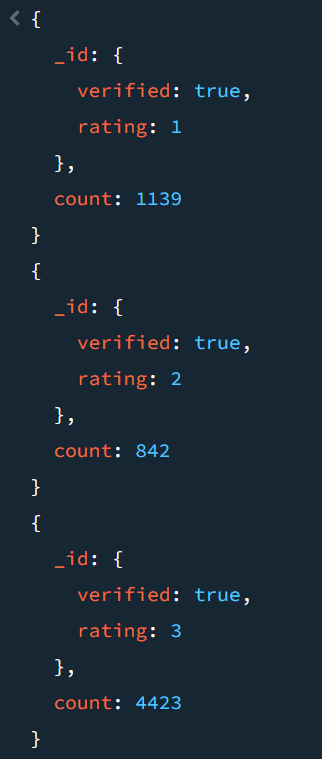
\includegraphics[width=0.7\textwidth]{Images/q6_result_1.png}
      \caption{Query 6 (partial) results for verified reviews}
  \end{minipage}\hfill
  \begin{minipage}{0.45\textwidth}
      \centering
      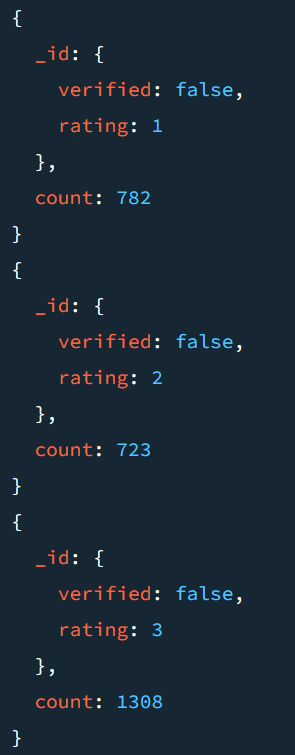
\includegraphics[width=0.65\textwidth]{Images/q6_result_2.png}
      \caption{Query 6 (partial) results for not verified reviews}
  \end{minipage}
\end{figure}
The number of reviews seems not to be so different between the two cases.
Anyway, if we consider the fact that, as shown in Figure \ref{fig:q6_result_spec}, the number of verified reviews is much higher, we can conclude that the percentage of low rating reviews is surely higher for the not verified ones. \\
\begin{figure}[H]
  \centering
  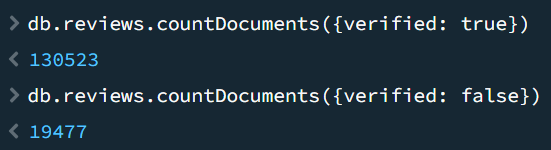
\includegraphics[scale=0.7]{Images/q6_result_spec.png}
  \caption{Number of verified and not verified reviews}
  \label{fig:q6_result_spec}
\end{figure}

\newpage
\subsection{Average Number of Votes for Verified vs. Non-Verified Reviews}
Another interesting query to compute can be the average number of votes for both verified and non verified reviews: this can be useful to understand if the fact that a review is verified or not has an impact on the number of votes that it receives. \\
\begin{lstlisting}[language=Java]
db.reviews.aggregate([
  { $group: { _id: "$verified", 
    avg_votes: { $avg: {$ifNull:[{$toInt: "$vote"}, 0]} } } }
]);
\end{lstlisting}
Results:
\begin{figure}[H]
  \centering
  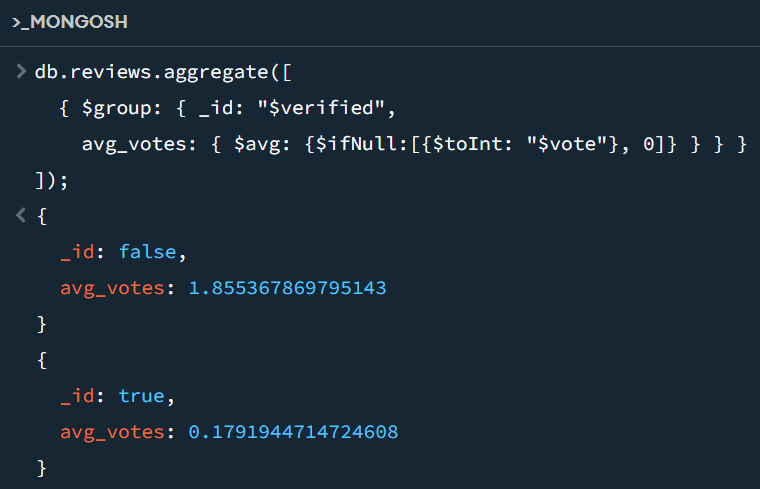
\includegraphics[scale=0.7]{Images/q7_result.png}
  \caption{Query 7 results}
  \label{fig:q7_result}
\end{figure}
As we can see from Figure \ref{fig:q7_result}, the average number of votes for non verified reviews is higher than the one for verified ones. 
Anyway, we don't think that this can be interpreted as a meaningful results since, like in the previous case, we also need to consider the over-abudance of verified reviews: it could be that since we used the \texttt{\$ifNull} operator to handle the case in which the \texttt{vote} field is missing, the average number of votes for verified reviews is lower because of the presence of many reviews with 0 votes.
This has been further investigated in Figure \ref{fig:q7_result_spec}. \\
\begin{figure}[H]
  \centering
  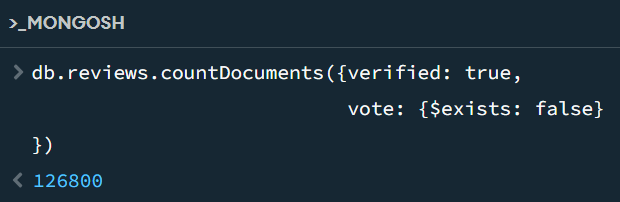
\includegraphics[scale=0.7]{Images/q7_result_spec.png}
  \caption{Number of verified reviews without the \textit{vote} field}
  \label{fig:q7_result_spec}
\end{figure}

\newpage
\subsection{Average Number of Votes for Low, Medium and High Rating Reviews}
To complete our investigation about which factors can influence the number of votes that a review receives, we can compute the average number of votes for both low and high rating reviews: this can be useful to understand if customers tend to trust more low or high rating reviews. \\
In order to do this we decided to consider two thresholds over the values of the \textit{overall} field in order to be able to classify the reviews as:
\begin{itemize}
    \item \textit{low rating}: if the value is less than 3;
    \item \textit{medium rating}: if the value is equal to 3;
    \item \textit{high rating}: if the value is greater than 3.
\end{itemize}
\begin{lstlisting}[language=Java]
db.reviews.aggregate([
  { $group: { _id: { $cond: [ { $lt: [ "$overall", 3 ] }, 
    "low", { $cond: [ { $eq: [ "$overall", 3 ] }, 
    "medium", "high" ] } ] }, 
    avg_votes: { $avg: {$ifNull:[{$toInt: "$vote"}, 0]} } } }
]);
\end{lstlisting}
As it can be seen, we used the \texttt{\$cond} operator to create the classification of the reviews based on their rating. \\
Results:
\begin{figure}[H]
  \centering
  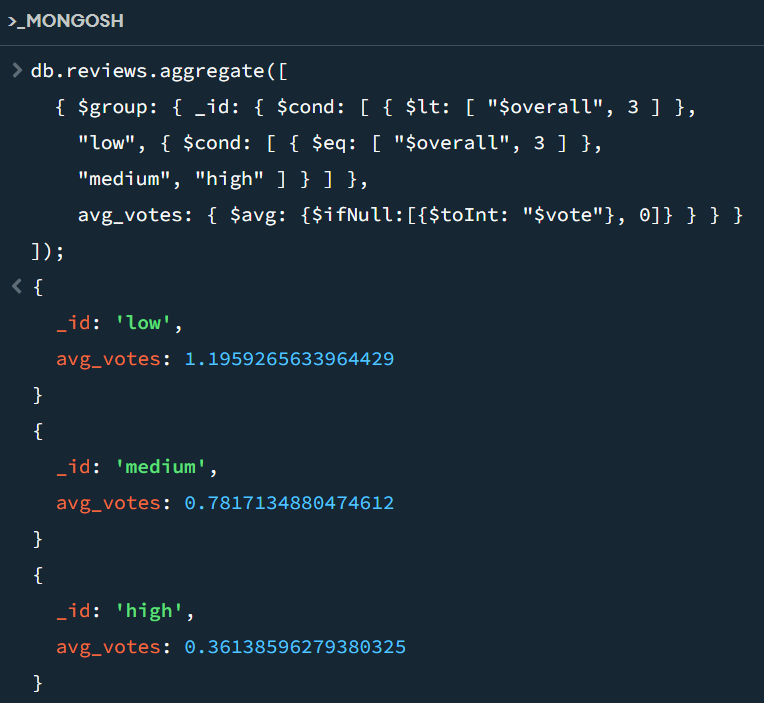
\includegraphics[scale=0.55]{Images/q8_result.png}
  \caption{Query 8 results}
  \label{fig:q8_result}
\end{figure}
Although it seems that people tend to trust a little more negative reviews, also in this case we don't know if we can draw any conclusion since we should consider the overall distribution of the ratings, which will be investigated in the next query. \\

\subsection{Distribution of Ratings}
In order to understand the distribution of the ratings, we can compute the number of reviews for every possible value of the \textit{overall} field. \\
\begin{lstlisting}[language=Java]
db.reviews.aggregate([
  { $group: { _id: "$overall", count: { $sum: 1 } } },
  { $sort: { _id: 1 } }
]);
\end{lstlisting}
Results:
\begin{figure}[H]
  \centering
  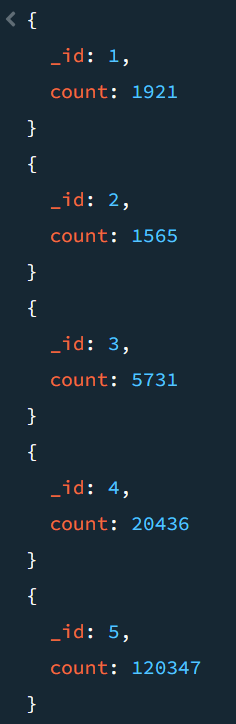
\includegraphics[scale=0.6]{Images/q9_result.png}
  \caption{Query 9 results}
  \label{fig:q9_result}
\end{figure}
As we can see from Figure \ref{fig:q9_result}, the number of reviews with a rating of 4 or 5 is much higher than the other ones.
We can understand multiple things from this:
\begin{itemize}
    \item in the context of the previous query, the number of high rating reviews is much higher than the number of low ones, so it can be possible that the average number of votes has been effected by the missing values in the \textit{vote} field for most of the high rating comments;
    \item people prefer to write positive reviews rather than negative ones.
\end{itemize}

\newpage
\subsection{Average Rating per Format Style and Year}
As our last query, we decided to compute the average rating for every possible value of the \textit{style.Format} field, in order to understand which was the most appreciated format style for every year. \\
\begin{lstlisting}[language=Java]
db.reviews.aggregate([
  { $match: {"style": {$exists: true}}},
  { $group: { _id: { year: { $year: { $toDate: {$multiply: [
          {
            "$toDecimal": "$unixReviewTime",
            
          },
          1000
        ]} } }, 
        format: "$style.Format:"}, 
      avg_rating: { $avg: "$overall" } } },
  { $sort: { "_id.year": 1, "avg_rating": -1} }
]);
\end{lstlisting}
Results:
\begin{figure}[H]
  \centering
  \begin{minipage}{0.45\textwidth}
      \centering
      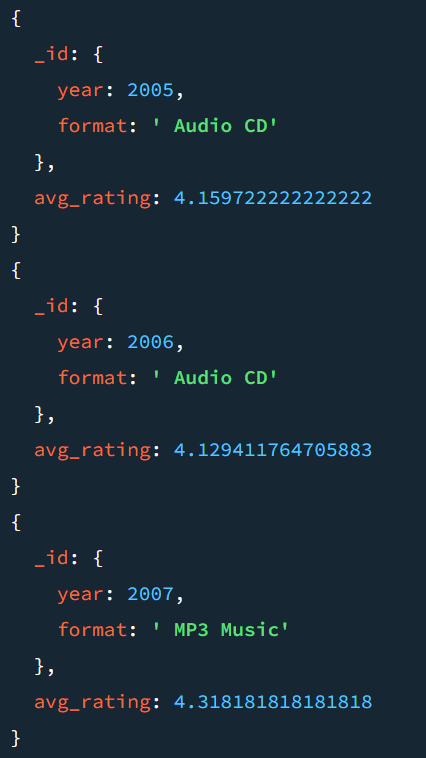
\includegraphics[width=0.7\textwidth]{Images/q10_result_1.png}
  \end{minipage}\hfill
  \begin{minipage}{0.45\textwidth}
      \centering
      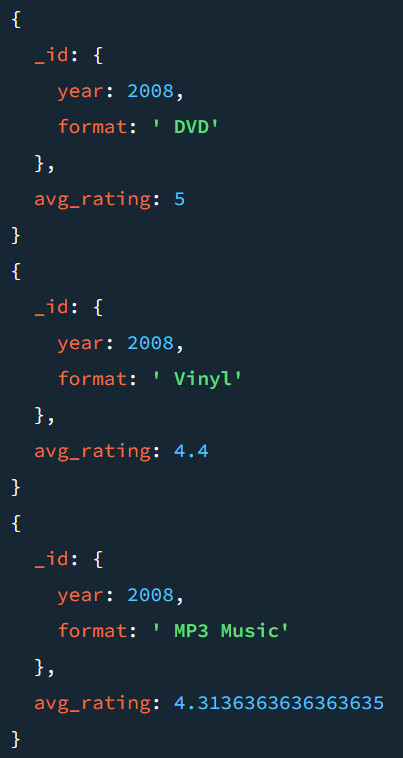
\includegraphics[width=0.65\textwidth]{Images/q10_result_2.png}
  \end{minipage}
  \caption{Query 10 (partial) results}
\end{figure}
This final query revealed many interesting things, such as the fact that \textit{Audio CD} has been the most appreciated format style for many years after the 1998, but in 2007 \textit{MP3 Music} took its place, probably because of the increasing popularity of digital music.
Another interesting fact can be seen in 2008, when \textit{DVD} was the most appreciated format style but \textit{Vinyl}, the oldest among all the considered formats, was in second place: this can be possibly explained by the fact that in that, from that year on, always more people became interested in old music and started using Amazon to buy these kind of products. \\
